% Kubernetes Scheduling Framework: extension points of one scheduling attempt.
% Used in blog/2025-08-24-guide-building-custom-kubernetes-scheduler.md
%
% Build (from web/):
%   cd diagrams && pdflatex scheduling-framework.tex
%   pdftocairo -svg scheduling-framework.pdf ../static/img/blog/scheduling-framework.svg
\documentclass[tikz,border=12pt]{standalone}
\usepackage[T1]{fontenc}
\usepackage{inter}
\renewcommand{\familydefault}{\sfdefault}
\usetikzlibrary{positioning,fit,backgrounds,calc,arrows.meta}

% Site palette
\definecolor{ink}{HTML}{1D1916}
\definecolor{muted}{HTML}{6E645B}
\definecolor{accent}{HTML}{B23A24}
\definecolor{band}{HTML}{F3ECE2}
\definecolor{rule}{HTML}{D8CFC3}

\begin{document}
\frenchspacing
\hyphenpenalty=10000
\exhyphenpenalty=10000
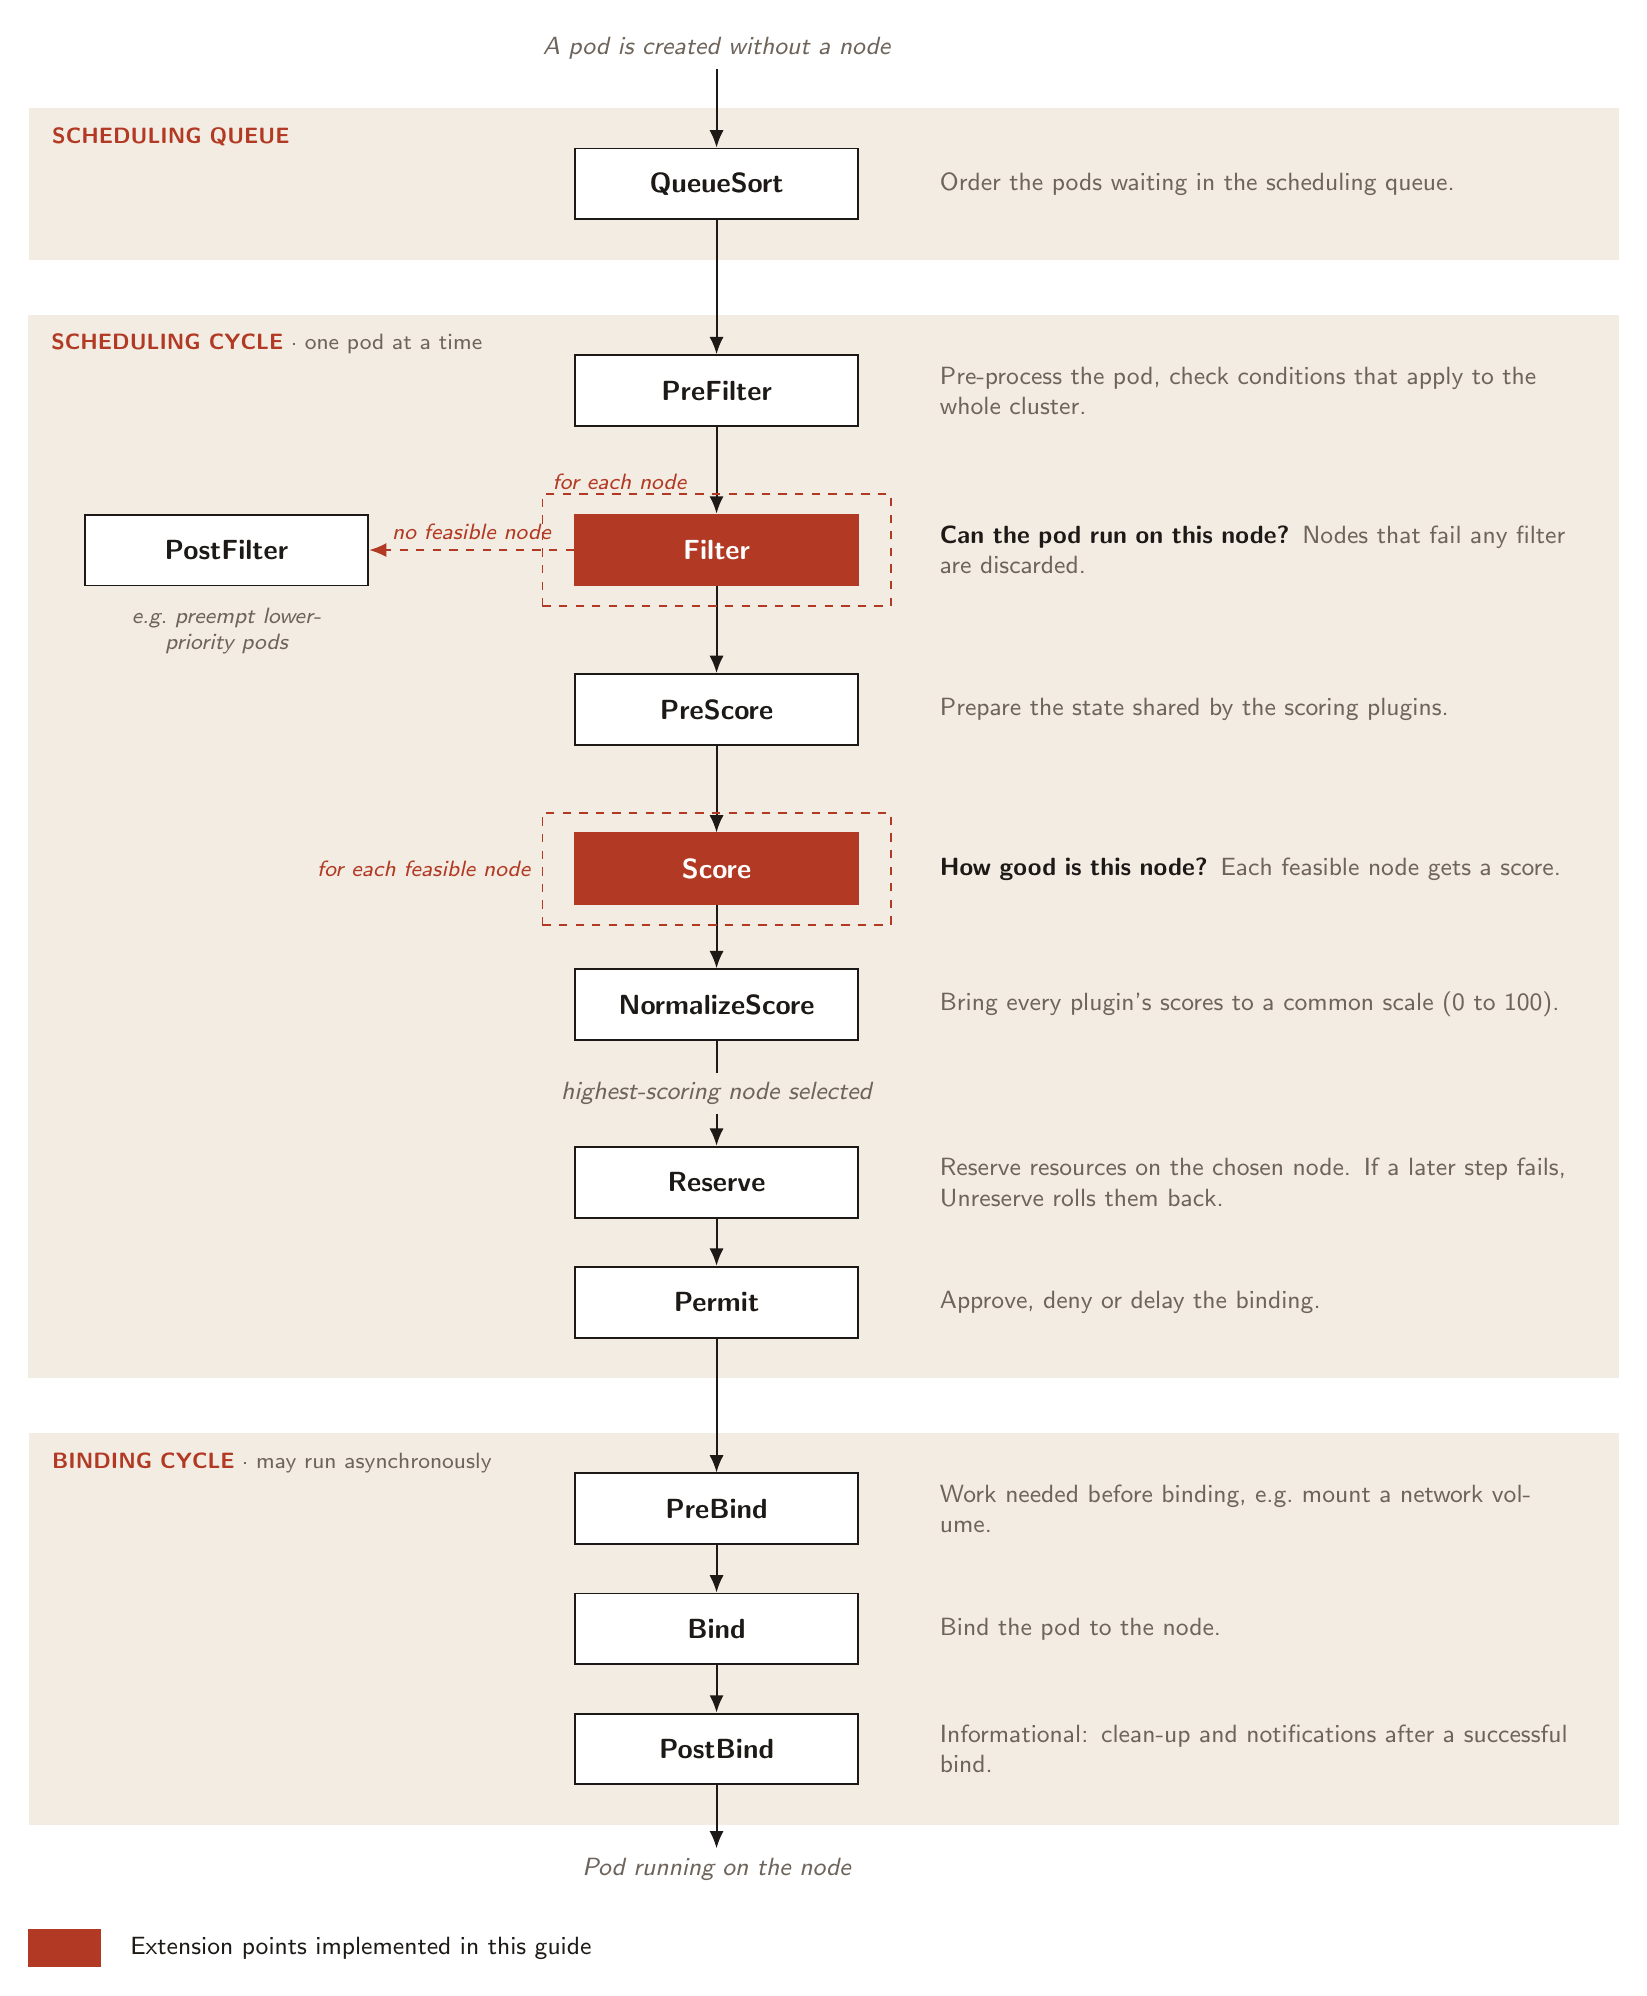
\begin{tikzpicture}[
    stage/.style={draw=ink, line width=0.7pt, fill=white, minimum width=36mm,
      minimum height=9mm, font=\bfseries, text=ink},
    hl/.style={stage, fill=accent, draw=accent, text=white},
    desc/.style={font=\small, text=muted, text width=80mm, align=left, anchor=west},
    note/.style={font=\small\itshape, text=muted},
    flow/.style={-{Latex[length=2.2mm,width=1.8mm]}, line width=0.7pt, draw=ink},
    branch/.style={flow, dashed, draw=accent},
    group/.style={fill=band, draw=none, inner sep=5mm},
    glabel/.style={font=\bfseries\footnotesize, text=accent, anchor=north west,
      inner sep=0pt, xshift=3mm, yshift=-2.5mm},
    loop/.style={draw=accent, dashed, line width=0.6pt, inner xsep=4mm, inner ysep=2.5mm},
    looplabel/.style={font=\footnotesize\itshape, text=accent, anchor=south west,
      inner sep=1pt, xshift=1mm},
  ]

  % ---------------------------------------------------------------- main flow
  \node[note] (start) {A pod is created without a node};
  \node[stage, below=10mm of start] (queuesort) {QueueSort};

  \node[stage, below=17mm of queuesort] (prefilter) {PreFilter};
  \node[hl, below=11mm of prefilter] (filter) {Filter};
  \node[stage, below=11mm of filter] (prescore) {PreScore};
  \node[hl, below=11mm of prescore] (score) {Score};
  \node[stage, below=8mm of score] (normalize) {NormalizeScore};
  \node[note, below=4mm of normalize] (pick) {highest-scoring node selected};
  \node[stage, below=4mm of pick] (reserve) {Reserve};
  \node[stage, below=6mm of reserve] (permit) {Permit};

  \node[stage, below=17mm of permit] (prebind) {PreBind};
  \node[stage, below=6mm of prebind] (bind) {Bind};
  \node[stage, below=6mm of bind] (postbind) {PostBind};
  \node[note, below=8mm of postbind] (end) {Pod running on the node};

  % ------------------------------------------------------------ side branch
  \node[stage, left=26mm of filter] (postfilter) {PostFilter};
  \node[note, font=\footnotesize\itshape, text width=38mm, align=center,
        below=1.5mm of postfilter] (postfilterdesc) {e.g.\ preempt lower-priority pods};

  % ------------------------------------------------------------ descriptions
  \node[desc, right=9mm of queuesort] (dqueuesort) {Order the pods waiting in the scheduling queue.};
  \node[desc, right=9mm of prefilter] (dprefilter) {Pre-process the pod, check conditions that apply to the whole cluster.};
  \node[desc, right=9mm of filter]    (dfilter)    {\textcolor{ink}{\textbf{Can the pod run on this node?}} Nodes that fail any filter are discarded.};
  \node[desc, right=9mm of prescore]  (dprescore)  {Prepare the state shared by the scoring plugins.};
  \node[desc, right=9mm of score]     (dscore)     {\textcolor{ink}{\textbf{How good is this node?}} Each feasible node gets a score.};
  \node[desc, right=9mm of normalize] (dnormalize) {Bring every plugin's scores to a common scale (0 to 100).};
  \node[desc, right=9mm of reserve]   (dreserve)   {Reserve resources on the chosen node. If a later step fails, Unreserve rolls them back.};
  \node[desc, right=9mm of permit]    (dpermit)    {Approve, deny or delay the binding.};
  \node[desc, right=9mm of prebind]   (dprebind)   {Work needed before binding, e.g.\ mount a network volume.};
  \node[desc, right=9mm of bind]      (dbind)      {Bind the pod to the node.};
  \node[desc, right=9mm of postbind]  (dpostbind)  {Informational: clean-up and notifications after a successful bind.};

  % ------------------------------------------------------------------ arrows
  \draw[flow] (start) -- (queuesort);
  \draw[flow] (queuesort) -- (prefilter);
  \draw[flow] (prefilter) -- (filter);
  \draw[flow] (filter) -- (prescore);
  \draw[flow] (prescore) -- (score);
  \draw[flow] (score) -- (normalize);
  \draw[line width=0.7pt, draw=ink] (normalize) -- (pick);
  \draw[flow] (pick) -- (reserve);
  \draw[flow] (reserve) -- (permit);
  \draw[flow] (permit) -- (prebind);
  \draw[flow] (prebind) -- (bind);
  \draw[flow] (bind) -- (postbind);
  \draw[flow] (postbind) -- (end);
  \draw[branch] (filter.west) -- node[above, font=\footnotesize\itshape, text=accent] {no feasible node} (postfilter.east);

  % ------------------------------------------------------------ loop markers
  \node[loop, fit=(filter)] (filterloop) {};
  \node[looplabel] at (filterloop.north west) {for each node};
  \node[loop, fit=(score)] (scoreloop) {};
  \node[looplabel, anchor=east, xshift=-2mm] at (scoreloop.west) {for each feasible node};

  % ------------------------------------------------------------------ groups
  \coordinate (left)  at ($(postfilter.west) + (-2mm,0)$);
  \coordinate (right) at ($(dfilter.east) + (0,0)$);

  \begin{scope}[on background layer]
    \node[group, fit=(left |- queuesort) (right |- queuesort) (queuesort) (dqueuesort)] (gqueue) {};
    \node[glabel] at (gqueue.north west) {SCHEDULING QUEUE};

    \node[group, fit=(left |- prefilter) (right |- permit) (prefilter) (permit) (postfilterdesc)
          (filterloop) (scoreloop) (dreserve)] (gcycle) {};
    \node[glabel] at (gcycle.north west) {SCHEDULING CYCLE \textcolor{muted}{\textmd{· one pod at a time}}};

    \node[group, fit=(left |- prebind) (right |- postbind) (prebind) (postbind) (dpostbind)] (gbind) {};
    \node[glabel] at (gbind.north west) {BINDING CYCLE \textcolor{muted}{\textmd{· may run asynchronously}}};
  \end{scope}

  % ------------------------------------------------------------------ legend
  \node[hl, minimum width=9mm, minimum height=4.5mm, anchor=west] (legendbox)
        at ($(gbind.south west |- end) + (0,-10mm)$) {};
  \node[font=\small, text=ink, anchor=west, right=2.5mm of legendbox]
        {Extension points implemented in this guide};
\end{tikzpicture}
\end{document}
